\section{La régression linéaire}
\label{chap4.section5}
La régression linéaire est l’un des modèles paramétriques les plus anciens, peut-être même le modèle fondamental de cette philosophie. Elle a été introduite au début du XIXe siècle par le mathématicien et statisticien Francis Galton, qui l'a utilisée pour étudier la relation entre la taille des parents et celle de leur progéniture. Depuis lors, la régression linéaire a été largement étudiée et appliquée dans divers domaines, notamment l’économie et, bien sûr, l’apprentissage automatique.

Le but de la régression linéaire est de créer une approximation de la relation linéaire entre chaque variable indépendante et la variable dépendante, celà sous-entend donc que pour que la régression linéaire soit efficace les prédicateurs doivent décrire une certaine forme de linéarité avec la variable dépendante, c'est-à-dire une corrélation non nulle entre les variables d'entrées et la sortie. Lorsqu’il n’y a qu’une seule variable indépendante, on qualifie la tâche de: \textbf{\textit{Régression linéaire simple ou univariée}}. Et régression linéaire multi-variée s'il y a plus d'une variable d'entrée. Formellement, le problème de la régression linéaire est donc le suivant:

Étant donné un ensemble de données décrivant une corrélation linéaire entre des prédicateurs \(x_i\) et une variable de sortie (target) \(y\); trouver les valeurs des paramètres \(w_i\) et \(b\) pour lesquels l'équation linéaire \(y_j = b + \Sigma_i w_i \cdot x_{j,i}\) est vraie ou sensiblement vraie pour chaque exemple \(x_j\) dans l'ensemble d'entrainement. Les \(w_i\) sont appélés les \textbf{poids} et \(b\) le \textbf{bias} du modèle. Pour trouver ces valeurs, on cherche à minimiser une \textbf{fonction de coût}.

\subsection{Fonction de coût}
\label{chap4.sec5.sub1}
Une fonction de coût est un moyen de mésurer et de pondérer l'erreur d'un modèle, on l'appelle aussi fonction de perte. Une fonction de perte \(L(y, \hat{y})\) est définie comme l'utilité perdue en prédisant \(h(x)= \hat{y}\) lorsque la bonne réponse est \(f(x) = y\). Une fonction de perte est différente d’un taux d’erreur, dans le sens où une fonction de perte ne s’intéresse pas seulement à l’erreur du modèle en prédisant \(\hat{y}\) au lieu de \(y\). Toute fonction qui capture la perte réelle résultant d'une mauvaise prédiction du modèle peut être une fonction de perte.

Prenons l'exemple de notre thème même, le risque encouru par l'institution prêteuse en accordant un prêt à une personne qui s'avère être un prêt défaillant est beaucoup plus grand que celui qu'elle encourt en refusant un prêt à quelqu'un qui aurait potentiellement pu le rembourser, raison pour laquelle certaines institutions durcissent leur critères sur les prêts et refusent beaucoup de demandes. Et pareil au niveau du client les risque ne sont pas les mêmes, donc un modèle qui prédit beaucoup trop souvent des défauts de paiement comme bon prêt causera plus de tort dans le monde réel qu'un autre modèle qui a le bias inverse. On peut faire une fonction de perte qui capture cette subtilité, c'est là la différence entre une fonction de coût et le taux d'erreur, par exemple on peut définir une fonction de coût de manière à ce que \(L(y=remboursera, \hat{y}=!remboursera)=1\) and \(L(y=!remboursera, \hat{y}=remboursera)=10\).

La fonction de coût est la mésure de performance de l'apprentissage supervisé car dans beaucoup d'algorithmes c'est elle que nous cherchons à minimiser. Pour expliquer les différents concepts impliqués dans l'entraînement de tels modèles dans le reste de ce document, nous allons nous baser sur une des formes les plus simples de fonction de coût, la fonction de perte \(L2\) ou perte quadratique qui est définie comme: \[L2(y, \hat{y}) = (y - \hat{y})^2\] Lors d'un entraînement nous cherchons à minimiser la somme totale des pertes sur l'ensemble des données d'entraînement soit: \[SumL2 = \Sigma_j (y_j - \hat{y}_j)^2\]

Dans le context de la régression linéaire, on le rappelle \(\hat{y}_j = b + \Sigma_i w_i \cdot x_{j,i}\), ce qui donne comme perte: \[SumL2 = \Sigma_j (y_j - (b + \Sigma_i w_i \cdot x_{j,i}))^2\]

Cette somme étant une équation avec \(i+1\) inconnues, pour chaque poids \(w_i\) et un bias \(b\), elle atteint sa valeur minimale quand les dérivées partielles de la somme par rapport à chacune des inconnues sont égales à 0. C'est-à-dire lorsque: \[\frac{\partial}{\partial w_i} \Sigma_j (y_j - (b + \Sigma_i w_i \cdot x_{j,i}))^2 = 0\] pour chaque \(w_i\) de l'ensemble des poids et \[\frac{\partial}{\partial b} \Sigma_j (y_j - (b + \Sigma_i w_i \cdot x_{j,i}))^2 = 0\]

Ces équations ont une seule solution unique (si elle existe), souvent celà implique que les valeurs idéales des poids et du bias sont des nombres réels avec plus de 50 décimales, leur calcul prend donc énormement de temps et on est souvent obligés de les tronquer de toute façon. Donc au lieu de chercher directement les solutions de ces équations on cherche à les approximer grâce à un algorithme qu'on appelle la \textbf{descente de gradient} qui est devenu la norme avec les modèles paramétriques. L'idée est que, par exemple, si les vraies valeurs de \(w_1\) et \(b\) pour que leurs dérivées partielles respectives soient exactement égales à zéro sont: $w_1 = 1,702145614785401$ et $b = -0,8745123177559741$. Eh bien, nous serions assez satisfaits d'un algorithme qui convergerait vers $w_1 = 1,701$ et $b = -0,874$.

\subsection{La Descente de gradient}
\label{chap4.sec5.sub2}
Avec la descente de gradient, les valeurs des paramètres sont initialisées « aléatoirement » avec de petites valeurs, généralement issues d'une distribution gaussienne ou tout simplement mises à zéro au début de l'algorithme et nous visons à converger par itération vers une approximation des valeurs optimales des poids et du bias qui minimise la fonction de coût. L'algorithme est le suivant:

Pour un certain nombre d'époques\footnote{Une époque d'entraînement réfère à une application de l'algorithme de descente de gradient sur l'ensemble d'entraînement entier.} d'entraînement ou tant que l'algorithme n'a pas encore convergé (ce qui signifie qu'il y a encore des changements importants dans les valeurs des paramètres), on calculera les « gradients », c'est-à-dire les dérivées partielle de la fonction de perte pour chaque paramètres et chaque exemple d'entraînement \(x_j\) et on mettra à jour les valeurs de chaque \(w_i\) et de \(b\) suivant la direction de leurs gradients. Formellement ça donne l'algorithme suivant:

Pour m de 1 à \(M\) nombre d'époques
\begin{enumerate}
    \item \textbf{Calculer les gradients}: Calculer les gradients de la fonction de perte par rapport à chaque paramètres.
    
    \begin{itemize}
        \item Pour un exemple d'entraînment \(x_j\) et un certain \(w_i\), poids du \(i\)ème attribut de \(x_j\) on a donc: \[\frac{\partial}{\partial w_i} L2 = \frac{\partial}{\partial w_i} (y_j - (b + w_i \cdot x_{j,i}))^2 = 2(y_j - (b + w_i \cdot x_{j,i})) \cdot \frac{\partial}{\partial w_i} (y_j - (b + w_i \cdot x_{j,i}))\] \[= -2(y_j - (b + w_i \cdot x_{j,i})) \cdot x_{j,i}\]
        \item Pour le bias on a: \[\frac{\partial}{\partial b} L2 = \frac{\partial}{\partial b} (y_j - (b + w_i \cdot x_{j,i}))^2 = 2(y_j - (b + w_i \cdot x_{j,i})) \cdot \frac{\partial}{\partial b} (y_j - (b + w_i \cdot x_{j,i}))\] \[= -2(y_j - (b + w_i \cdot x_{j,i}))\]
    \end{itemize}
    
    Pour trouver les expressions ci-dessus il est juste nécéssaire de connaître les bases de la différentiation telles que: \(\frac{\partial}{\partial w} wx = x\) et \(\frac{\partial}{\partial w} w = 1\)
    
    \item \textbf{Mettre à jour les valeurs des paramètres}: Ensuite l'algorithme mettra à jour les valeurs des paramètres en utilisant la règle suivante:
    
    \begin{itemize}
        \item Pour chaque \(w_i\): \[w_i \leftarrow w_i - \eta \cdot \frac{\partial}{\partial w_i} L2\]
        \item Pour le bias: \[b \leftarrow b - \eta \cdot \frac{\partial}{\partial b} L2\] où \(\eta\) est le taux d'apprentissage, même principe que celui de la section \ref{chap4.sec4.sub1}
    \end{itemize}
    
\end{enumerate}

Une forme plus complète de l'algorithme est obtenu en sommant les mises à jours des poids pour chaque exemple d'entraînement \(x_j\) par rapport à la somme des pertes. Ce qui donne, pour \(j\) de 1 à \(N\) nombre d'exemples:

\begin{itemize}
    \item Pour chaque \(w_i\): \[w_i \leftarrow w_i - \eta \cdot \Sigma_j \frac{\partial}{\partial w_i} SumL2 = w_i + 2\eta \cdot \Sigma_j^N (y_j - (b + w_i \cdot x_{j,i})) \cdot x_{j,i}\]
    \item Pour \(b\): \[b \leftarrow b - \eta \cdot \Sigma_j \frac{\partial}{\partial b} SumL2 = b + 2\eta \cdot \Sigma_j^N (y_j - (b + w_i \cdot x_{j,i}))\]
\end{itemize}

En pratique, au lieu de répeter ces opérations pour chaque prédicateurs (donc pour chaque \(w_i\), ce qui va s'avérer très lent, on va plutôt vectorialiser toutes les équations précédentes depuis l'équation de prédiction du modèle. Ce qui va donner:

\begin{itemize}
    \item L'équation du modèles devient: \[\hat{Y} = b + W \cdot X\] où $W$ est la matrice des poids où \(w_{j,i}\) est le poids associé au $i$ème attribut du $j$ème exemple d'entraînement, \(X\) est la matrice de tous les exemples d'entraînement avec tous les prédicateurs, cette matrice est de la même forme que $W$, le bias reste une valeur unique pour tout l'ensemble et $\hat{Y}$ est le vecteur des prédictions sur l'ensemble entier, de manière similaire \(Y\) est le vecteur des vraies étiquettes.
    \item La formule de mise à jour des poids par la descente de gradient devient: \[W \leftarrow W - \eta \cdot \frac{\partial}{\partial W} SumL2 = W + 2\eta \cdot (Y - (b + W \cdot X)) \cdot X\] où \(W\) sera une matrice dont on pourra prendre la moyenne ou la somme par colonne comme nouvelle valeur des \(w_i\)
    \item La formule de mise à jour du bias par la descente de gradient devient: \[b \leftarrow b - \eta \cdot \frac{\partial}{\partial b} SumL2 = b + 2\eta \cdot (Y - (b + W \cdot X))\] où $b$ sera une matrice de bias dont on pourra ensuite prendre la moyenne ou la somme comme valeur unique pour $b$. Notez aussi que la plupart du temps on simplifie \(2\eta\) à \(\eta\) tout simplement car le taux d'apprentissage est généralement un nombre très petit dont la multiplication par 2 reste semblable à ce dernier.
\end{itemize}

En répétant donc le processus ci-dessus pour \(M\) iteration sur l'ensemble de données entier, \(M\) époque, l'algorithme de descente de gradient va converger vers les valeurs de chaque paramètres pour lesquelles la somme des pertes est minimiser. Il est plus facile de raisonner avec les formes simples de ces équations qu'avec leur formes matricielles donc pour les prochaines démonstration où on aura besoin de revenir à ces équations j'utiliserai les formes simples. La figure \ref{fig:fig7} montre une illustration d'un modèle de régression linéaire univariée entraîner pour prédire le prix d'une maison avec une seule variable indépendante qui est sa superficie. On peut voir que le modèle, alors définie par juste un poids et un bias, décrit une droite qui correspond presque parfaitement aux données d'entraînement et qui peut être utilisé pour prédire une estimation du prix d'une nouvelle maison. L'idée pour les modèles multi-variée aussi est de trouver les valeurs des paramètres de l'hyperplan\footnote{En géométrie, un hyperplan est une généralisation d'un plan bidimensionnel dans un espace tridimensionnel à des espaces mathématiques de dimension arbitraire. Comme un plan dans l'espace, un hyperplan est une hypersurface plate, un sous-espace dont la dimension est inférieure d'une unité à celle de l'espace ambiant. Dans un espace bidimensionnel, c'est une ligne; dans un espace tridimensionnel, c'est un plan, et ainsi de suite.} qui décrit le même comportement pour un espace multi-dimensionnel.

\begin{figure}
    \centering
    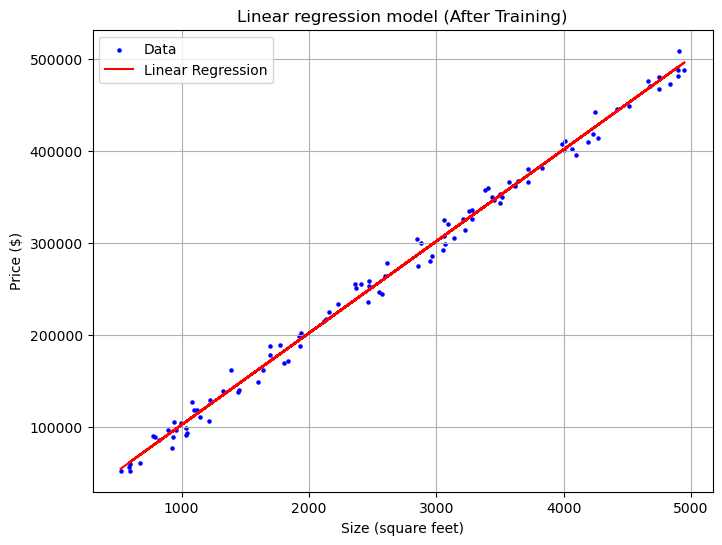
\includegraphics[width=0.75\linewidth]{images/linreg.png}
    \caption{Un modèle de régression linéaire simple décrit une droite qui suit la relation linéaire de l'ensemble de données}
    \label{fig:fig7}
\end{figure}

Tout comme pour les arbres de décisions je n'ai pas implémenté de modèle de régression linéaire pour ce projet. Comme son nom l'indique la régression linéaire est un algorithme de régression et la tâche de prédire les défauts de paiement est une tâche de classification, cependant expliquer la régression linéaire en profondeur comme ici me permettra d'être plus concis dans les explications des trois dernier modèles que j'ai testé.